\documentclass[12pt,a4paper]{report}
\usepackage[utf8]{inputenc}
\usepackage[francais]{babel}
\usepackage[T1]{fontenc}
\usepackage{amsmath}
\usepackage{amsfonts}
\usepackage{amssymb}
\usepackage{graphicx}
\usepackage{lmodern}
\usepackage{setspace}
\usepackage{float}
\usepackage{fancyhdr} 
\usepackage{footnote}
\usepackage{array}
\usepackage[title,titletoc,toc]{appendix}
\usepackage{hyperref}

\hypersetup{
    colorlinks,
    citecolor=black,
    filecolor=black,
    linkcolor=black,
    urlcolor=black
}

\author{Baptiste Lesquoy}
\title{Rapport d'initiation à la recherche}

\begin{document}




\thispagestyle{empty}

\begin{minipage}{.5\textwidth}%haut gauche
\begin{figure}[H]
\includegraphics[scale=1.2]{resources/logoUniv.jpg}
\end{figure}
\end{minipage}
%
\begin{minipage}{.5\textwidth}%haut droite
\begin{flushright}
Master Informatique\\
Promotion 2015-2017
\end{flushright}
\end{minipage}

\begin{center}
\vspace{\stretch{7}}
{\huge Localisation de robot} \\
\vspace{\stretch{1}}
\textbf{Rapport d'initiation à la recherche}\\
\vspace{\stretch{7}}
\end{center}

\begin{minipage}{.5\textwidth}%bas gauche
Travail effectué en\\
mai 2016\\ 
sous la direction de\\
Dmitry Sokolov
\end{minipage}
%
\begin{minipage}{.5\textwidth}%bas droite
\begin{flushright}
Présenté par\\
Baptiste Lesquoy\\
\end{flushright}
\end{minipage}

\setcounter{page}{0}
\newpage

\tableofcontents

\part{Le sujet}
\chapter{Étude du problème}

\section{Objectif général}
Dans le cadre de la coupe de France de robotique, on aimerait pouvoir localiser un robot. On entend par localisation, le fait de retrouver, avec plus ou moins de précision, sa position sur le terrain.
On prendra l'exemple du terrain de l'édition 2016, mais dans l'absolu la solution doit pouvoir fonctionner ailleurs. L'environnement étant connu à l'avance, on ne cherchera pas ici à construire une carte de celui-ci, mais uniquement à se positionner sur une carte déjà construite. De plus on cherchera à avoir une solution le plus économique possible. Enfin, même si on travaillera la plupart du temps sur le même robot, la solution apportée ne doit pas être spécifique à ce dernier, il s'agit d'une méthode, d'un protocole plus que d'une implémentation.

\section{Les solutions de localisations existantes}
Pour localiser un robot, il existe de nombreuses techniques. La plus utilisée est certainement l'odométrie, c'est à dire la mesure mouvements des roues (ou chenilles) pour recréer le mouvement du véhicule. Cette technique permet en effet, à partir des données des moteurs (puissance, durée ...) d'avoir une bonne approximation du mouvement effectué. Le problème de l'odométrie est que certains déplacements du véhicules sont impossible à mesurer simplement avec ces données. Par exemple si le véhicule glisse, il se sera déplacé sans même que les roues ne tournent. Ainsi on couple souvent l'odométrie avec les données d'autres capteurs, par exemple un capteur ultrason pour détecter les objets proche. Ce qui permet de corriger les éventuelles erreurs. 

Parmi les techniques couramment employées, on retrouve aussi toutes celles qui ont pour principe de se repérer en calculant sa position par rapport à d'autres éléments connus. Par exemple avec des caméras on peut évaluer la distance qui nous sépare d'un objet particulier (une sorte de balise) et en déduire notre position. C'est un peu la même chose pour le système GPS, où le récepteur calcule sa position grâce au temps qu'ont mis les messages des satellites à lui arriver.

Il existe autant de techniques que de situation, mais aucune n'est fiable à 100 pourcent. C'est pourquoi de manière générale on essaye le plus possible d'en combiner plusieurs, afin de recouper les données.

\section{Solutions applicables dans le contexte ?}

Suivant le contexte, certaines techniques sont plus appropriées que d'autres. Il a donc fallu définir quelles étaient les contraintes qu'imposait la coupe de France de robotique, et quelles techniques y répondaient le mieux.

Premièrement la compétition se déroule en intérieur et les dimensions du terrain sont très réduites (2m sur 3m), il est donc impossible d'utiliser un système de positionnement satellite.

On pourrait utiliser un système de caméra pour se déplacer, mais généralement ce genre de méthodes demandent beaucoup de ressources pour être utilisées correctement. Or les systèmes embarqués sont peu puissant. De plus, la reconnaissance d'éléments en 3D est un domaine qui est loin d'être maîtrisé.  C'est donc une piste possible, mais où la difficulté pour arriver à un système réellement utilisable est faible.

L'odométrie convient très bien, seulement comme il a été dit précédemment, elle ne permet pas d'être sûr de sa position. La coupler avec une autre méthode peut être une solution.

On peut aussi utiliser le principe de la localisation par GPS, mais l'adapter à la taille du terrain. Les règles de la coupe de France indiquent que chaque équipe dispose de 3 supports fixe autour du terrain qui peuvent servir d'emplacement pour des balises. On peut donc imaginer poser des lumières ou des enceintes à ces emplacements, et se repérer grâce à eux. Pour les lumières la difficulté est que l'environnement est très lumineux, et qu'en plus si on veut qu'elle soit visible, il faut les placer en hauteur (pour ne pas être gêné par les autres robots ou les objets sur le terrain). Donc le capteur qui devra les regarder regardera vers le haut, c'est à dire vers les lampes au plafond. Pour le son, c'est un peu le même problème, la coupe de France de robotique est très bruyante, il y a de la musique en continu, des commentateurs avec des micros et le public autour.

Néanmoins c'est cette dernière solution (la localisation à l'aide d'enceintes) que nous avons choisi. En effet, bien qu'il semble difficile de la mettre en place à cause du bruit ambiant, cela n'est pas impossible. De plus c'est une des seules solutions qui apporte quelque chose de nouveau, les autres étant déjà régulièrement utilisées (avec plus ou moins de succès). Enfin le coût de mise en œuvre ne semble à priori pas très élevé, puisqu'il suffit d'avoir quelques enceintes et des micros. On partira du principe que cette méthode pourra être couplée à une autre dans la pratique, même si on se concentrera uniquement sur celle-ci.


\begin{figure}[H]
\includegraphics[width=13cm]{resources/img/terrain_officiel.png} 
\caption{le terrain officiel de l'édition 2016 de la coupe de France de robotique (détaillé dans le règlement\cite{reglement_cdf}}
\end{figure}

\chapter{Three Omnidirectional Sound Beacons de John Swindle: Une méthode proche de la notre}
Il s'agit d'un article de John Swindle\cite{john_swindle2010} dans lequel il détaille son implémentation d'un système qui semble correspondre à ce que nous cherchons à réaliser: la localisation d'un robot à l'aide du son. On tâchera donc de comprendre la solution qu'il a apporté, puis de la modifier pour l'adapter à nos propres contraintes.


\subsection{Fonctionnement de son système}
Le système qu'il décrit fonctionne à l'aide de 3 enceintes synchronisées et un micro.

Prenons l'exemple de l'image ci-dessous. Le robot a reçu les sons dans cet ordre: A, puis B, puis C.
le robot (M) ne connait pas la distance qui le sépare de A qu'on note $r_{m}$. Par contre il sait combien de temps sépare sa réception du son de A de celle du son de B. Ce temps représente donc le temps que le son a pris pour parcourir la distance qui le sépare de B moins $r_{m}$. On peut convertir ce temps en distance car on connait la vitesse de déplacement du son dans l'air, on note cette distance $d_{1}$. Il nous reste à répéter l'opération pour le son suivant et on trouve la distance $d_{2}$.

\begin{figure}[H]
\includegraphics[width=15cm]{resources/img/fonctionnement_gps.png} 
\caption{schéma de fonctionnement du système: en rouge le robot, en bleu les enceintes. Illustration prise dans l'article de John Swindle\cite{john_swindle2010}}
\end{figure}

Il nous reste donc juste à résoudre le système d'équation généré (détaillé dans l'article\cite{john_swindle2010}) pour trouver la position du micro. 

Pour que cela marche il faut qu'on sache où chaque enceinte se trouve.
Il faut aussi que les 3 enceintes émettent exactement en même temps.


\subsection{Problèmes du système et idées de solutions}
Le problème de ce système pour l'utilisation qu'on veut en faire est qu'il requiert que les enceintes émettent exactement en même temps (ou au moins avec un décalage fixe et connu). Or cela implique que les 3 enceintes, qui se trouvent des deux côtés opposés du terrain soit contrôlées par un même ordinateur, que l'ordinateur dispose d'un amplificateur pour gérer les 3 enceintes (habituellement les cartes sons en gèrent 2 maximum) le tout devant partager un des support de 8cm * 8cm * 16cm avec une des enceinte. En plus de cela se pose le problème de la liaison entre les différentes balises. Bien qu'il soit autorisé de le faire par câble, c'est peu pratique, et il est possible que le signal soit bruité ou en retard car il faut utiliser plus de 4 mètres de câble pour relier un côté à l'autre. Par ondes (wifi/bluetooth ...) les problèmes sont les même en plus accentués au niveau du signal et on peut ajouter à cela la possibilité de perdre la connexion ou d'avoir des interférences avec l'environnement (par exemples les téléphones portable dans la pièce).
On aimerait donc pouvoir se passer de la synchronisation des enceintes.

La solution trouvée est simple: chacune des enceintes a un signal propre et émet sans aucun contrôle extérieur. Cette fois au lieu de mesurer le décalage entre la réception de deux signaux, on va mesurer le décalage d'un même signal en deux points connus. Il faudra donc un robot équipé de 2 micros. 


\part{Travail effectué}
\chapter{Objectif}

L'objectif de ce projet était dans un premier temps de vérifier si la technique de localisation élaborée était utilisable, et si oui dans quelle mesure (matériel nécessaire, précision etc.). Et ensuite si possible commencer à implémenter certaines parties de cette technique. Enfin, pour les parties ne pouvant être implémentées, il faudrait fournir des pistes de réflexions pour les prochains à travailler dessus.

\chapter{Viabilité de la technique}
Une très grande partie du projet a consisté à tester la viabilité de la technique. On a commencé par vérifier que le matériel qu'on utilisait était fiable(les micros côte à côte reçoivent le même signal, la mousse isolante réduit l'intensité du signal ...), puis on a continué en vérifiant certaines propriétés qui nous semblaient importante.\\

À commencer par le fameux décalage de phase qui servait de base au projet. Nous avons testé si on pouvait bien observer un déphasage entre deux micro et surtout si on pouvait retrouver à partir de là la vrai distance séparant les micros. Les résultats ont été concluant, on arrive à retrouver les distances physiques à partir des décalages observés avec une bonne précision. L'idée est donc exploitable.\\

Nous avons ensuite continué en observant l'influence de l'écho sur le signal reçu, et nous avons pu constater que selon le niveau d'écho on pouvait avoir de grosses variations. Pour éviter cela nous avons émis l'hypothèse qu'en entourant le micro de mousse on pouvait filtrer une partie de l'écho. Ce qui s'est avéré correct.\\

Enfin nous avons effectués des tests afin de vérifier que les signaux envoyés étaient reconnaissable une fois enregistré, et nous avons essayé de déterminer quel type de signal conviendrait le mieux à notre problématique. Pour ce qui est de reconnaitre le signal envoyé, il n'y a pas eu de problème particulier, sauf pour les signaux continu long qui devenaient difficile à reconnaitre quand l'écho venait s'ajouter. Ce problème peut être résolu simplement en utilisant un signal de type sinusoïdal, puisque l'écho va simplement agrandir le sinus. Mais après plusieurs essaies nous avons opté pour une répétition de signaux brefs, car ces derniers sont trop court pour être perturbé par de l'écho, et plus facilement reconnaissable dans un environnement bruyant.\\

\begin{figure}
\includegraphics[width=15cm]{../tests/lecture_de_signaux_carres/donnees11-03/test_2.jpg}
\caption{Illustration: photo d'une mesure du décalage entre 2 micros alignés}
\end{figure}

Toutes ces expériences ont été réalisé plusieurs fois et dans des configurations différentes afin d'être sûr que les résultats étaient reproductible. Chacune d'elle a fait l'objet d'un rapport détaillé où le maximum d'informations sur le contexte de l'expérience on été fournies afin qu'elles puissent être reproduite ou que les résultats puissent être jugés par des personnes extérieurs.

\chapter{Implémentation}

Une fois le projet jugé viable, nous nous sommes lancé dans une phase d'implémentation, dans l'espoir de fournir une preuve de concept.

On peut découper la réalisation d'un système fonctionnel en 3 parties. Pour commencer il y a la partie qui nettoie le signal reçu afin de mettre en évidence le décalage de phase. Ensuite y a la partie principale, celle qui permet à partir de 3 décalage de phase de déterminer où se trouve le robot. Enfin il y a l'automatisation/ la reconnaissance automatique du signal envoyé. Le temps disponible étant assez limité il a été décidé de faire l'impasse sur la partie automatisation dès le début. Ainsi durant l'implémentation, on simulera cette partie en faisant la reconnaissance/automatisation nous même.


\section{Traitement du signal}
Afin de nettoyer le signal reçu pour ne retrouver qu'un "clac" envoyé, on utilise une technique très simple. Il suffit de prendre la période à laquelle sont envoyé chaque "clac", de découper le signal reçu en bouts de la taille de cette période, et d'additionner le tout. De cette manière on va amplifier tout ce qui se répète suivant la même période, en l'occurrence les clacs, et le reste étant plus ou moins aléatoire, s'annule au fur et à mesure des additions.
Avec cette méthode on obtient de bons résultats tant que le bruit ambiant n'est pas trop important, mais ça ne fonctionne plus à partir d'un certain niveau de bruit.

Une chose qui aurait pût être traitée aussi, mais qui ne l'a pas été par manque de temps est la différenciation des signaux selon de quel enceinte ils viennent.

\section{Retrouver la position du robot}

Pour cette partie, il a été décidé de reproduire les conditions de la coupe de France de robotique et de voir si on été capable à partir d'un enregistrement de retrouver la position à laquelle se trouvaient les micros.\\
Pour commencer il a fallu créer un terrain aux dimensions proches, puis d'y marquer les différents emplacements des enceintes et des micros, afin de pouvoir reproduire l'expérience.\\
\begin{figure}[H]
\includegraphics[width=15cm]{resources/img/terrain.jpg}
\caption{Le terrain construit avec les marques des différents emplacements}
\end{figure}

Les micros ont été fixé à de la mousse des deux extrémités d'une baguette de bois, afin de simuler le support sur lesquels ils seront placé en conditions réelles.
\begin{figure}[H]
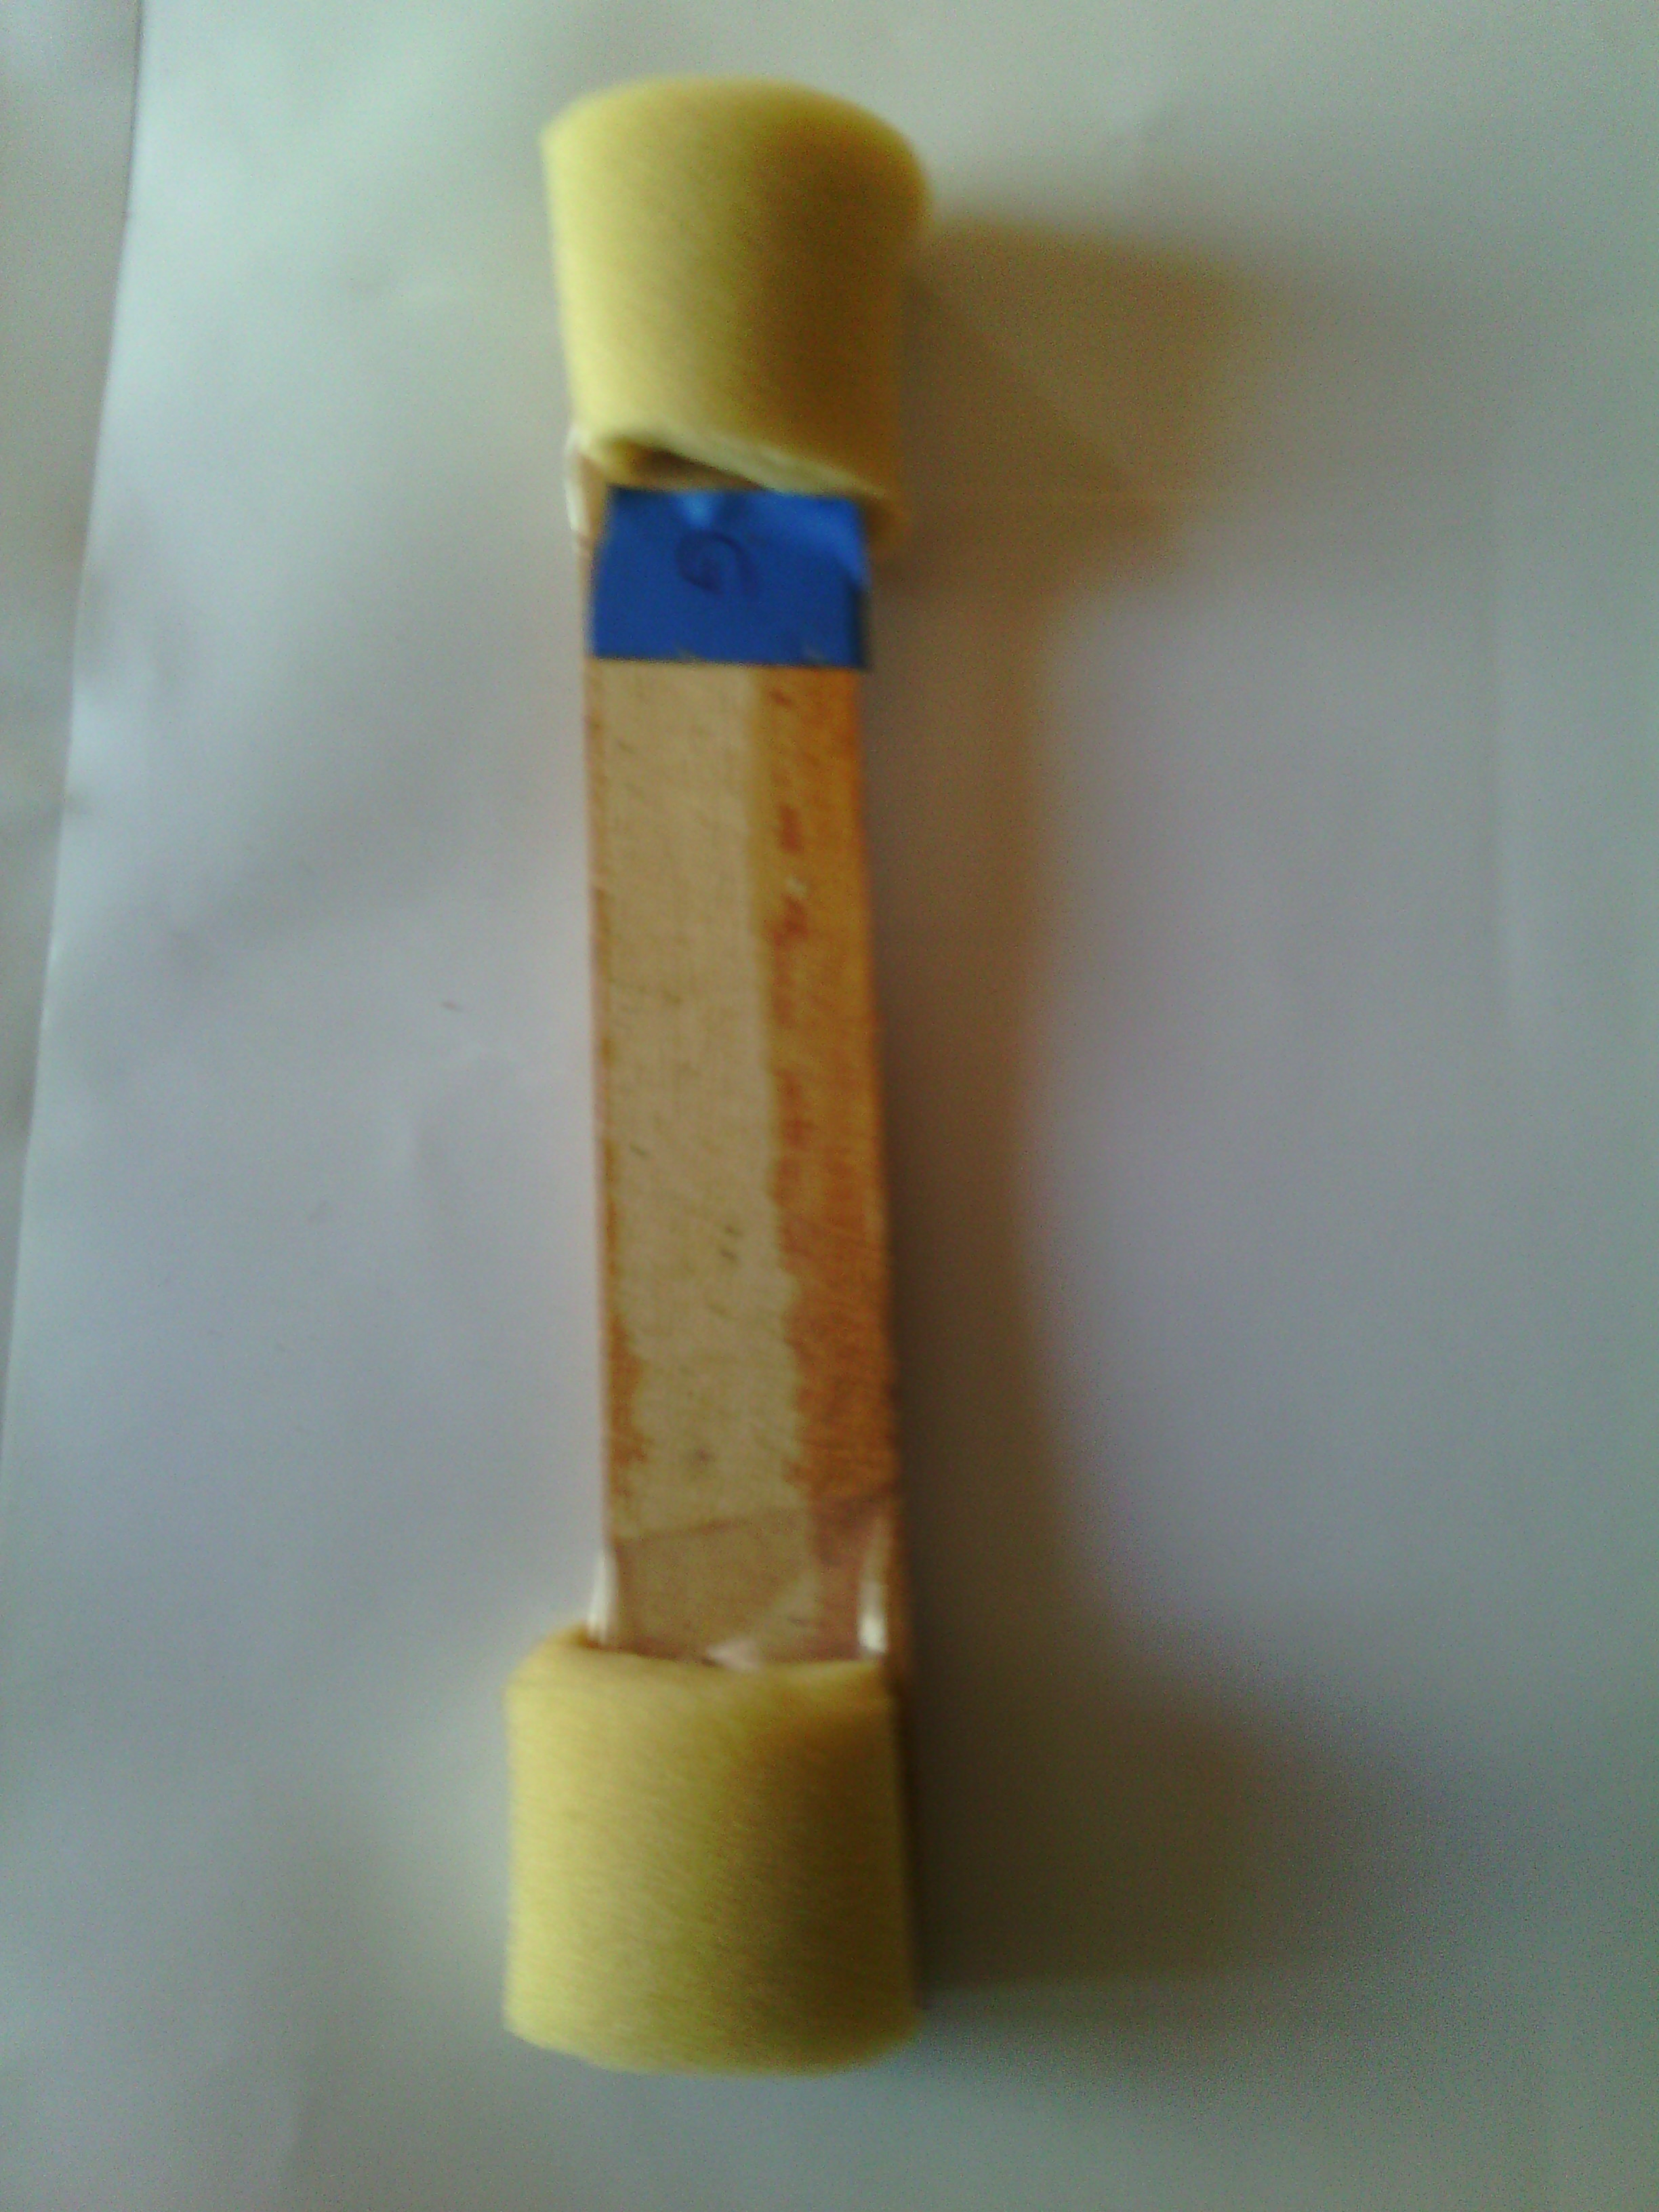
\includegraphics[width=8cm]{resources/img/micros.png}
\caption{le support des micros}
\end{figure}

Finalement pour chacun des 6 emplacements on a pris 3 mesures par enceinte.\\
Une fois ces données recueillies il fallait trouver un moyen à partir des décalages de retrouver la position des micros. Utiliser simplement les équations du système ne nous donnera pas forcément une réponse car il se peut que les données soit légèrement différentes de la réalité, et que donc les équations n'aient pas de solution. \\
C'est pourquoi il a été décidé de modéliser le terrain, et de juger chacune des positions possible en fonction des décalage qu'on est censé y observer par rapport à ceux enregistrés. Ainsi la ou les positions dont les décalages sont le plus proche de ceux observés obtiendra/ont la meilleur note.\\
On  peut donc créer une carte représentant le terrain, où chaque pixel aurait une couleur associé à son score.
\begin{figure}[H]
\includegraphics[width=15cm]{../tests/simu_coupe_de_france_a_la_main/P2.png}
\caption{Le score de chaque position sur le terrain en fonction de sa proximité avec P2. les points les plus noir ont le meilleur score}
\end{figure}
On obtient de manière très visuelle une idée d'où se trouve le robot.
En observant un peu les cartes générés, on remarque qu'il peut y avoir plusieurs zones bien distinctes possible. On en conclu que cette méthode doit être couplé à une autre afin de pouvoir départager entre ces zones. Par exemple, comme à chaque position on a associé un angle (pas visible sur la figure car ça implique une représentation 3D moins compréhensible), connaitre la réelle orientation à l'aide d'un gyroscope pourrait permettre de supprimer beaucoup d'ambiguïté. On pourrait aussi s'aider des positions précédentes du robot pour décider.


\part{Conclusion}

Le système semble répondre aux critères initiaux: il est peu coûteux( 3 enceintes et 2 micros), il permet de se repérer sur une carte (bien que le coupler avec un autre système ou multiplier les mesures semble nécessaire), il est utilisable dans le cadre de la coupe de France de robotique et il est applicable à n'importe quel robot.

Les parties restant à développer pour avoir un système complet sont donc l'automatisation de la reconnaissance du signal émis dans le signal reçu, et la différenciation des signaux venant des différentes enceintes dans le signal reçu. Pour cette dernière partie, le problème est que quand on filtre un signal qui contient plusieurs "clac" d'enceintes différentes, peut importe avec la période de quel clac on filtre, on retrouve les traces très marqués des autres. Pour en venir à bout il est peut être possible d'étendre la méthode d'addition de période. En effet lorsqu'on cherche le "clac" à une fréquence particulière on pourrait en plus soustraire le spectre des "clac" aux autres fréquences. Une autre idée serait de mettre des temps mort variable d'une enceinte à l'autre entre chaque vague de "clac", ainsi, avec des valeurs choisie judicieusement on limiterait le nombre de superposition de signaux au même moment. 

Enfin lors de ce projet nous nous sommes intéressé uniquement au positionnement sur une carte plate, il serait intéressant de voir s'il est possible avec cette méthode de se positionner en 3 dimensions.


\bibliographystyle{plain}
\bibliography{resources/biblio}

\end{document} 